% Options for packages loaded elsewhere
\PassOptionsToPackage{unicode}{hyperref}
\PassOptionsToPackage{hyphens}{url}
\PassOptionsToPackage{dvipsnames,svgnames*,x11names*}{xcolor}
%
\documentclass[
  11pt,
]{article}
\usepackage{amsmath,amssymb}
\usepackage{lmodern}
\usepackage{ifxetex,ifluatex}
\ifnum 0\ifxetex 1\fi\ifluatex 1\fi=0 % if pdftex
  \usepackage[T1]{fontenc}
  \usepackage[utf8]{inputenc}
  \usepackage{textcomp} % provide euro and other symbols
\else % if luatex or xetex
  \usepackage{unicode-math}
  \defaultfontfeatures{Scale=MatchLowercase}
  \defaultfontfeatures[\rmfamily]{Ligatures=TeX,Scale=1}
  \setmainfont[]{CharisSIL}
\fi
% Use upquote if available, for straight quotes in verbatim environments
\IfFileExists{upquote.sty}{\usepackage{upquote}}{}
\IfFileExists{microtype.sty}{% use microtype if available
  \usepackage[]{microtype}
  \UseMicrotypeSet[protrusion]{basicmath} % disable protrusion for tt fonts
}{}
\makeatletter
\@ifundefined{KOMAClassName}{% if non-KOMA class
  \IfFileExists{parskip.sty}{%
    \usepackage{parskip}
  }{% else
    \setlength{\parindent}{0pt}
    \setlength{\parskip}{6pt plus 2pt minus 1pt}}
}{% if KOMA class
  \KOMAoptions{parskip=half}}
\makeatother
\usepackage{xcolor}
\IfFileExists{xurl.sty}{\usepackage{xurl}}{} % add URL line breaks if available
\IfFileExists{bookmark.sty}{\usepackage{bookmark}}{\usepackage{hyperref}}
\hypersetup{
  pdftitle={Week 8 Forced Alignment},
  pdfauthor={Hywel Stoakes \textbar{} Experimental Phonetics},
  colorlinks=true,
  linkcolor=blue,
  filecolor=Maroon,
  citecolor=Blue,
  urlcolor=Blue,
  pdfcreator={LaTeX via pandoc}}
\urlstyle{same} % disable monospaced font for URLs
\usepackage[margin=1in]{geometry}
\usepackage{graphicx}
\makeatletter
\def\maxwidth{\ifdim\Gin@nat@width>\linewidth\linewidth\else\Gin@nat@width\fi}
\def\maxheight{\ifdim\Gin@nat@height>\textheight\textheight\else\Gin@nat@height\fi}
\makeatother
% Scale images if necessary, so that they will not overflow the page
% margins by default, and it is still possible to overwrite the defaults
% using explicit options in \includegraphics[width, height, ...]{}
\setkeys{Gin}{width=\maxwidth,height=\maxheight,keepaspectratio}
% Set default figure placement to htbp
\makeatletter
\def\fps@figure{htbp}
\makeatother
\setlength{\emergencystretch}{3em} % prevent overfull lines
\providecommand{\tightlist}{%
  \setlength{\itemsep}{0pt}\setlength{\parskip}{0pt}}
\setcounter{secnumdepth}{-\maxdimen} % remove section numbering
\ifluatex
  \usepackage{selnolig}  % disable illegal ligatures
\fi

\title{Week 8 Forced Alignment}
\author{Hywel Stoakes \textbar{} Experimental Phonetics}
\date{2021-04-26}

\begin{document}
\maketitle

{
\hypersetup{linkcolor=}
\setcounter{tocdepth}{2}
\tableofcontents
}
\hypertarget{project-setup}{%
\section{Project Setup}\label{project-setup}}

\begin{enumerate}
\def\labelenumi{\arabic{enumi}.}
\tightlist
\item
  Once you have download and upzip this project:
\end{enumerate}

\begin{itemize}
\tightlist
\item
  (\url{https://github.com/Hywel-Stoakes/Forced_Alignment_Workshop})
\end{itemize}

\begin{enumerate}
\def\labelenumi{\arabic{enumi}.}
\setcounter{enumi}{1}
\item
  navigate to Canvas (LMS) and download the zip file called
  \texttt{W8\_data.zip} Copy the unzipped files to the \texttt{data}
  directory within the project folder.
\item
  Be sure to be running a Chrome Browser (available here:
  \url{https://www.google.com/chrome/})
\end{enumerate}

\hypertarget{open-rstudio}{%
\subsection{Open Rstudio}\label{open-rstudio}}

\begin{enumerate}
\def\labelenumi{\arabic{enumi}.}
\setcounter{enumi}{3}
\tightlist
\item
  Now open Rstudio (or double click the .Rproj in the root of the
  folder).
\end{enumerate}

\hypertarget{forced-alignment-of-australian-english}{%
\section{Forced Alignment of Australian
English}\label{forced-alignment-of-australian-english}}

In this section of the workshop we are going to automatically segment
some read speech from the ANDOSL corpus of Australian English. You are
probably all very familiar with these examples by now. We will be using
an Audio file (wav) and an associated text file with a transcript of the
speech in English orthography.

The Output will be a textgrid with the words segmented and also the
phones force aligned based on the orthographic input.

There a number of flavours of WebMAUS and the BAS tools generally and we
will look at some of the others in some detail and give you an idea of
the sort of files you may need before you start.

\hypertarget{navigate-to-webmaus-basic}{%
\subsection{Navigate to WebMAUS Basic}\label{navigate-to-webmaus-basic}}

First we will look at the WebMAUS Basic tool using a web browser and
then we will continue to look at alternative ways to access the MAUS
system.

\begin{enumerate}
\def\labelenumi{\arabic{enumi}.}
\tightlist
\item
  Open the Chrome Browser
\item
  You can navigate to \textbf{WebMAUS Basic} Here :
\end{enumerate}

\begin{itemize}
\tightlist
\item
  \url{https://clarin.phonetik.uni-muenchen.de/BASWebServices/interface/WebMAUSBasic}
\end{itemize}

\hypertarget{input-for-webmaus-basic}{%
\subsection{Input for WebMAUS Basic}\label{input-for-webmaus-basic}}

To use WebMAUS you will need:

\begin{itemize}
\tightlist
\item
  An \textbf{Audio} (\texttt{wav}) file (note that you can use a variety
  of file types as input including compressed formats such as
  \texttt{mp3}/\texttt{mp4} and other formats such as \texttt{aiff}).
\item
  An \textbf{Annotation} file as a text tile (\texttt{txt}) (note:
  WebMAUS also accepts \texttt{docx}/\texttt{pdf} and other formats.
  Note that this method doesn't allow \texttt{TextGrids} as input).
\end{itemize}

\hypertarget{how-to-get-some-output-for-webmaus-basic}{%
\subsection{How to get some output for WebMAUS
Basic}\label{how-to-get-some-output-for-webmaus-basic}}

\begin{enumerate}
\def\labelenumi{\arabic{enumi}.}
\item
  Drag and drop pairs of files to the dotted rectangle. (see figure 1.)

  \begin{itemize}
  \tightlist
  \item
    we will input the files from \texttt{"data/andosl\_text"} (drag and
    drop them all)
  \end{itemize}
\item
  Then click the \texttt{Upload} Button
\item
  In \textbf{Service Options} Change \textbf{Language} to
  \texttt{English\ (AU)} and \textbf{Output format} to
  \texttt{Praat\ (TextGrid)}
\end{enumerate}

\begin{figure}
\centering
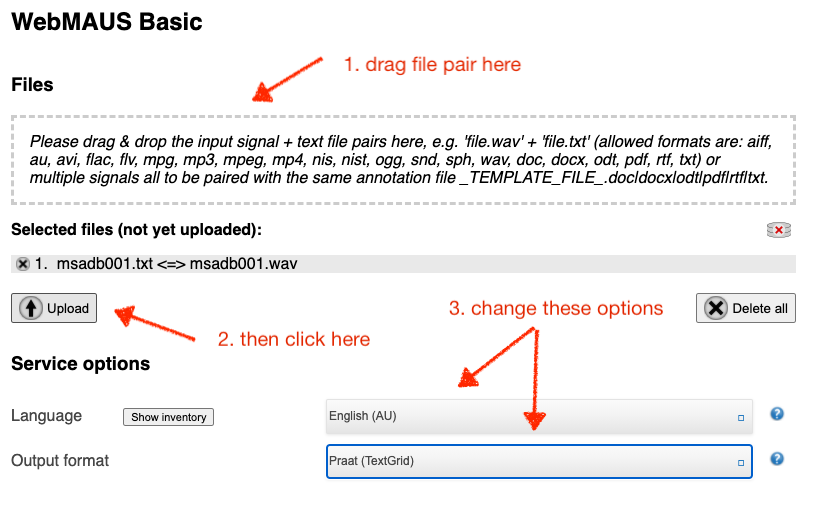
\includegraphics{/Users/hywel/Dropbox (Personal)/Teaching/2021_ExpPhon/Week_8/Forced_Alignment_Workshop/figures/WebMAUSBasicII.png}
\caption{webmaus\_basic options}
\end{figure}

\begin{enumerate}
\def\labelenumi{\arabic{enumi}.}
\setcounter{enumi}{3}
\tightlist
\item
  Then under the \textbf{Run} heading, click the box that indicates that
  you agree to the \emph{Terms of Usage} and click the
  \texttt{Run\ Web\ Service} button (see figure 2.)
\end{enumerate}

\begin{figure}
\centering
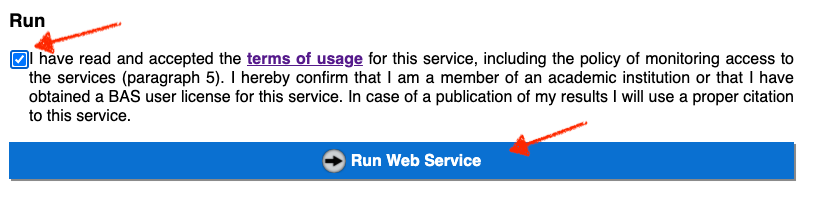
\includegraphics{/Users/hywel/Dropbox (Personal)/Teaching/2021_ExpPhon/Week_8/Forced_Alignment_Workshop/figures/WebMAUSBasicIII.png}
\caption{run webmaus}
\end{figure}

\hypertarget{output-from-webmaus-basic}{%
\subsection{Output from WebMAUS Basic}\label{output-from-webmaus-basic}}

Once you click the run button there will be a dialogue box with some
tips and tricks for the WebMAUS service that appear and a progress bar
along the top of the browser window.

\begin{figure}
\centering
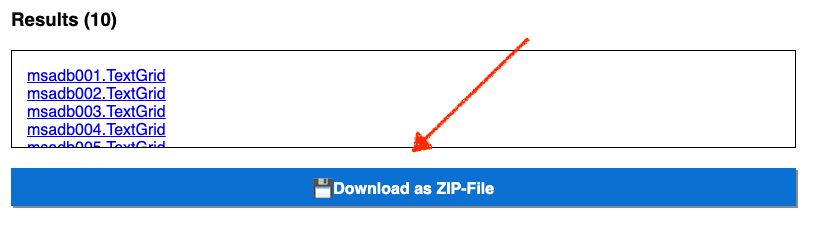
\includegraphics{/Users/hywel/Dropbox (Personal)/Teaching/2021_ExpPhon/Week_8/Forced_Alignment_Workshop/figures/WebMAUSoutput.png}
\caption{webmaus output}
\end{figure}

If the service has been successful the message box at the bottom of the
window will go green and you will get an option to
\texttt{Download\ as\ a\ ZIP-file}. If you get a yellow warning message
you still may be able to retrieve results. If the warning shows a red
box however there may be an error that has prevented any out put. It is
for this reason that it is best to split up large numbers of files into
smaller groups.

\begin{figure}
\centering
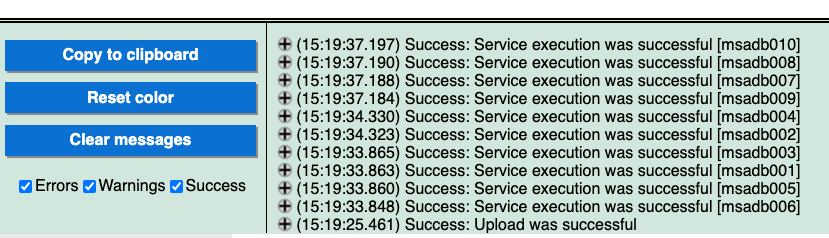
\includegraphics{/Users/hywel/Dropbox (Personal)/Teaching/2021_ExpPhon/Week_8/Forced_Alignment_Workshop/figures/WebMAUSbox.png}
\caption{webmaus messages}
\end{figure}

The resulting zip file will have a file name that is in the form:
\texttt{results-2021-04-26\_06-11-09.zip}. This will contain the
TextGrid files, unzip this folder and open the files in \texttt{Praat}.
You will need to find the original wav files (in
\texttt{data/andosl\_text}) and copy them to the results folder. You
should now see that there are 3 tiers in the textgrid: One called
\texttt{ORT-MAU}, the next called \texttt{KAN-MAU} and the bottom tier
called \texttt{MAU}. The \texttt{MAU} extension on the tier name shows
that they have been force aligned rather than hand-labelled.

\end{document}
